\documentclass[11pt]{beamer}
\usepackage[utf8]{inputenc}
\usepackage[T1]{fontenc}
\usepackage{lmodern}
\usepackage[spanish]{babel}
\usepackage{amsmath}
%%\usepackage{hyperref}
\usepackage{amsfonts}
\usepackage{amssymb}
\usepackage{graphicx}
\usepackage{epstopdf}
\usetheme{Frankfurt}
\usepackage{tikz}
\usetikzlibrary{patterns}
\usetikzlibrary{plotmarks}
\titlegraphic{\vspace{8cm}}% to push the other text to the top
\begin{document}
	\author{
		Departamento de Investigacion en F\'isica \\
		Maestría en Ciencias (Física)\\
		Hiram Ernesto Dami\'an}
	\title{Search for production of a Higgs boson and a single top quark in $\mu\mu$ final states in proton collisions at $\sqrt{s}=13$ TeV}
	%\subtitle{}
	\logo{
\includegraphics[scale=0.1]{unison-logo.png}}
	\institute{Universidad de Sonora}
	%\date{}
	%\subject{}
	\newcommand{\subf}[2]{%
		{\small\begin{tabular}[t]{@{}c@{}}
				#1\\#2
		\end{tabular}}%
	}
	%\setbeamercovered{transparent}
	%\setbeamertemplate{navigation symbols}{}
	\begin{frame}
	\titlepage
\end{frame}

\begin{frame}
\tableofcontents
\frametitle{Contenido}
\end{frame}


\begin{frame}
\section{Overview}
\frametitle{Overview}
\begin{itemize}
\item Through this project we will investigate the production of Higgs boson in association with a
single top quark (tH) in proton-proton collisions with the CMS experiment of the LHC. This
mechanism of production of the Higgs boson has not been observed before by any
experiment.

\item Understanding the production of the Higgs boson, as well as its decays are an important part
of the physical program of the CERN international laboratory experiments that try to complete
the tests to verify the Standard Model, the theory of the fundamental particles

\end{itemize}
\end{frame}


\begin{frame}
\subsection{Motivation}
\frametitle{Motivation  for single top Higgs (tH)}
\begin{itemize}
\item Coupling measurement is essential to establish the nature of the Higgs
\item The exploration of Higgs production on the tH channel is subject relatively new
\item The tHq study explores the relative sign of top-Higgs and W-Higgs
\item Measurements of CMS and ATLAS are compatible with SM.
\item Small deviations from SM predictions could be associated with physics beyond the
standard model (BSM)
\end{itemize}
\end{frame}

\begin{frame}
\section{tH mechanisms}
\frametitle{Higgs production mechanisms}
\begin{center}
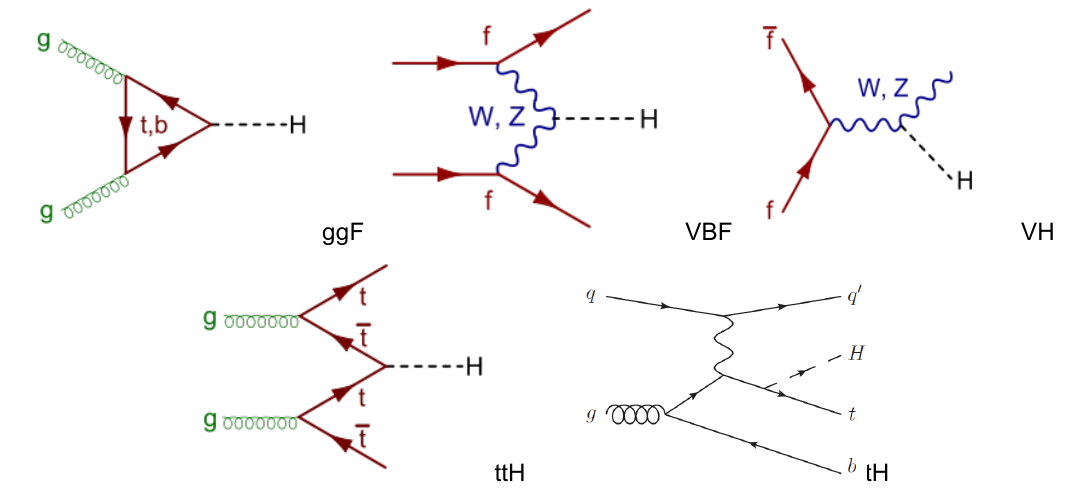
\includegraphics[scale=0.4]{figures/pg.png}
\end{center}
\end{frame}

\begin{frame}
\frametitle{tH production mechanisms}
\begin{center}
\begin{figure}
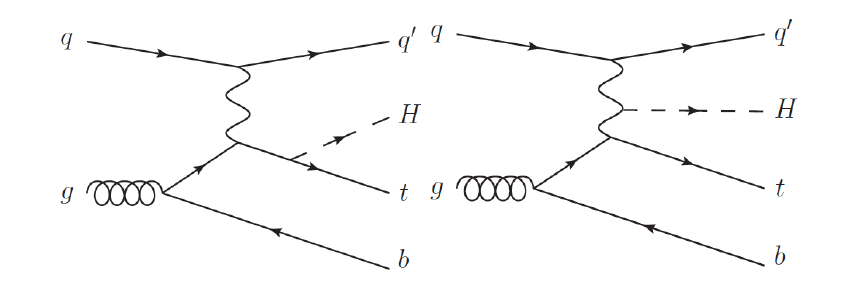
\includegraphics[scale=0.4]{figures/tq.png}
\caption{th mechanism. Left. Higgs from a top quark. Right.Higgs from a W boson}
\end{figure}
\end{center}
\end{frame}

\begin{frame}
\section{Cross section}
\frametitle{Cross section}
\begin{itemize}
\item When two particles interact, cross section is the area transverse to their relative motion within
which they must meet in order to scatter from each other.
\item Scattering cross sections may be defined as collisions of accelerated beams of one type of
particle with targets (either stationary or moving) of a second type of particle
\item cross section describes the likelihood of two particles interacting under certain conditions(2)
\end{itemize}

Experimentally
\begin{align}
d\sigma=\frac{\text{Number of particles scattered into solid angle} \Delta\Omega}{\text{(number of particles incident)(scattering centers/area)}}
\end{align}
\end{frame}

\begin{frame}
\frametitle{Cross section}
\begin{center}
	\begin{figure}
		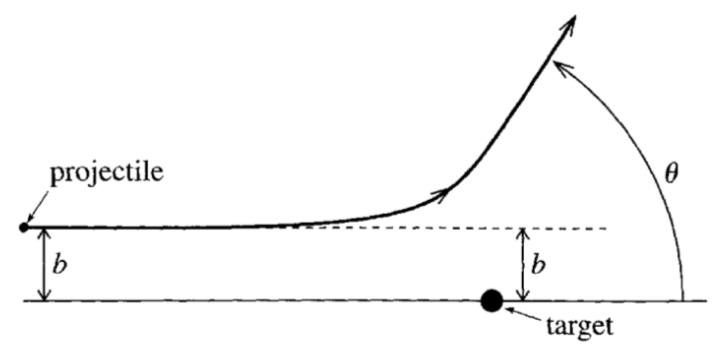
\includegraphics[scale=0.5]{figures/cs.png}
		\caption{Drawing of an idealized scattering process showing the differential solid angle $\Delta\Omega$ and the
			scattering angle $\theta$}
	\end{figure}
\end{center}
\end{frame}

\begin{frame}
\frametitle{Cross section}
Higgs boson production cross sections and uncertainties as a function of the pp collider energy (in
pico barn)\footnotemark.\\

\begin{tabular}{|c|c|c|}
\hline

Production mechanism &
$\sigma$ (picobarns pb)
&Number of events \\
\hline
ggF &
48.61&
1745099\\
\hline
VH &
13.73&
492907\\
\hline
VBF &
1.378&
1357738\\
\hline
ttH &
0.507&
17745\\
\hline
tH	 (only)&
0.0742&
2663.78\\
\hline
\end{tabular}


\footnotetext[1]{\tiny{Data taken from The cern collaborarion “Higgs Physics the HL-LHC and HE-LHC” 2019, CERN-LPCC-2018-04}}

\end{frame}

\begin{frame}
\frametitle{Cross section}
\begin{center}
\begin{figure}
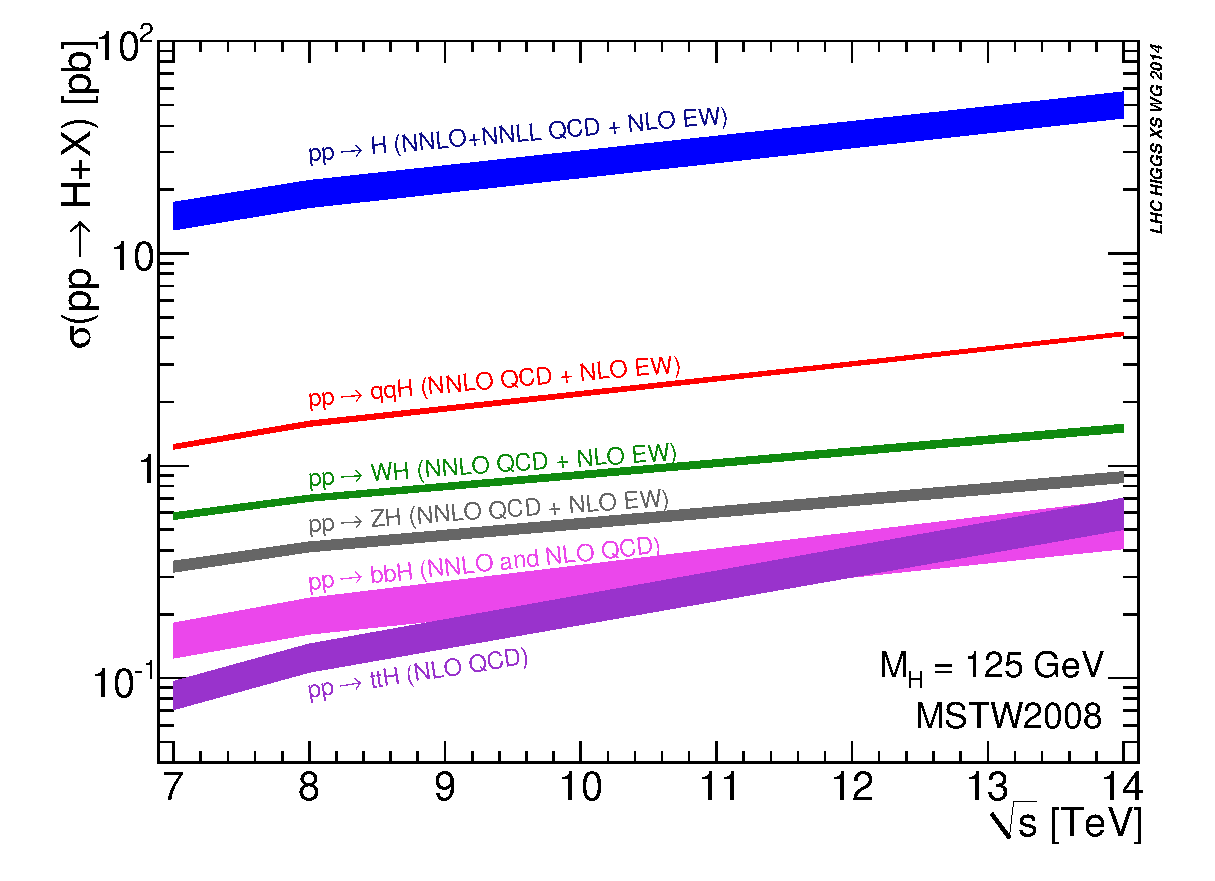
\includegraphics[scale=0.42]{figures/7-14xsec.eps}
\caption{Standard Model Higgs boson production cross sections at Ecm = 13 and 14 TeV as a function of Higgs boson
	mass and Higgs boson production cross sections as a function of the centre-of-mass-energies
}	
\end{figure}
\end{center}
\end{frame}



\begin{frame}
\frametitle{Cross section}
\begin{center}
	\begin{figure}
		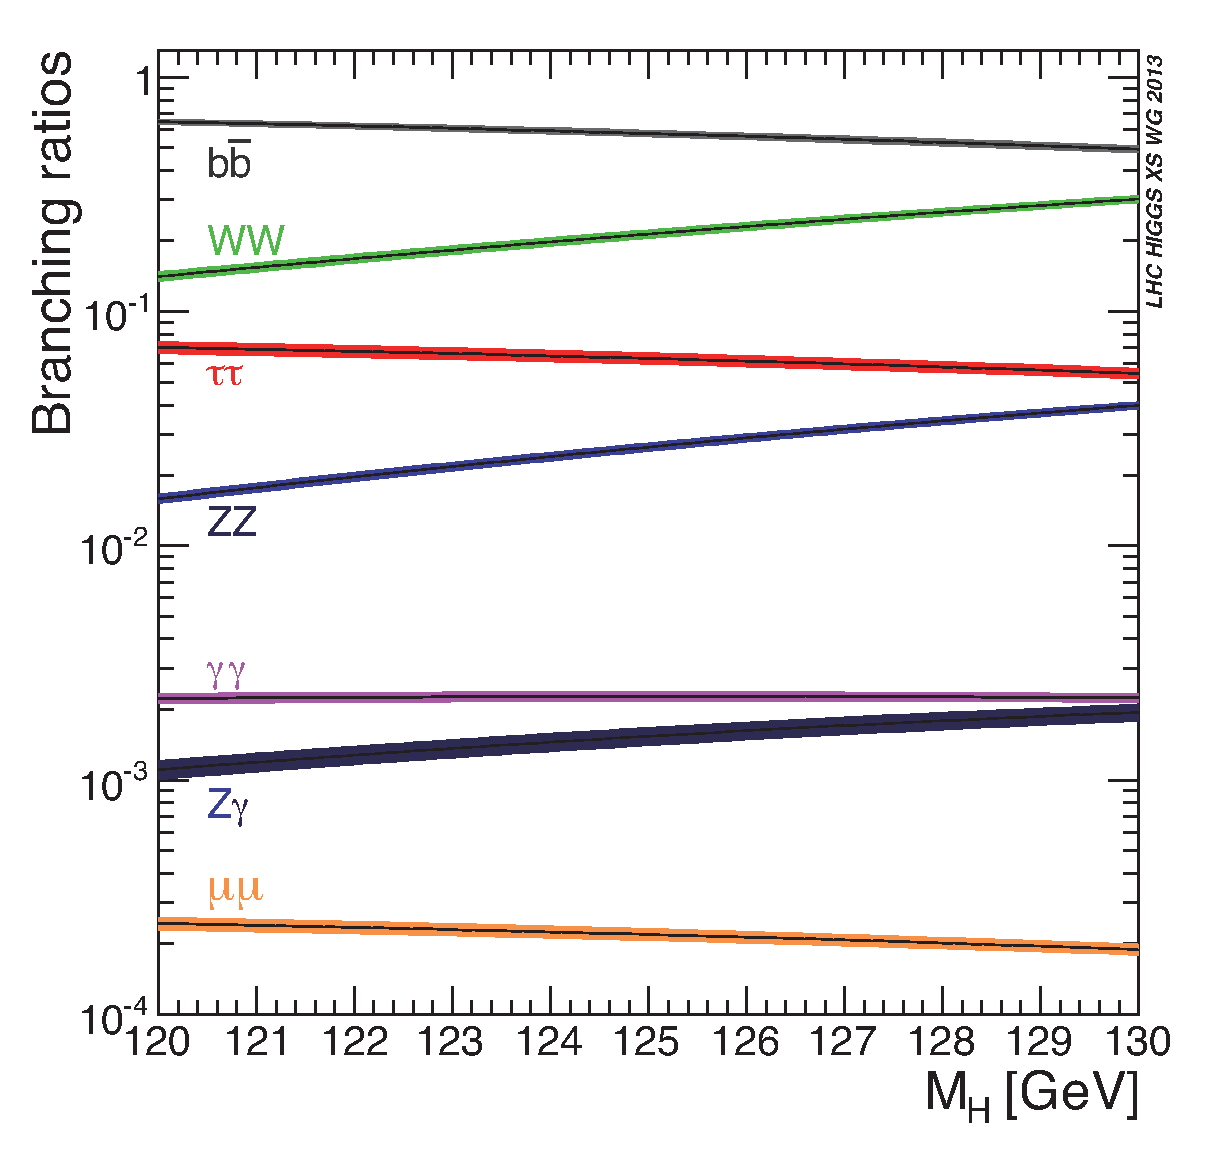
\includegraphics[scale=0.42]{figures/Higgs_BR_120-130_7.eps}
		\caption{Standard Model Higgs boson decay branching ratios and total width}	
	\end{figure}
\end{center}
\end{frame}


\begin{frame}
\section{Higgs Branching ratios and expected events per channel}
\frametitle{Higgs Branching ratios and expected events per channel}
SM Higgs boson branching ratios and number of events per decay for tH process $M_H$ =125 GeV\\
\begin{center}
\begin{tabular}{|c|c|}
	\hline
	Higgs decay & Branching ratio (BR)\\
	\hline
	H $\rightarrow$ b$\bar{b}$ &
	$5.82\times 10^{-1}$ \\
	\hline
	H $\rightarrow$ $W^+W^-$ &
	$2.15\times10^{-1}$ \\
	\hline
	H $\rightarrow$ $\tau^+\tau^-$ &
	$6.27\times10^{-2}$\\
\hline
	H $\rightarrow$ ZZ &
$2.61\times10^{-2}$\\
\hline
	H $\rightarrow$ $\gamma\gamma$ &
$2.27\times10^{-3}$\\
\hline
	H $\rightarrow$ Z$\gamma$ &
$1.53\times10^{-3}$\\
\hline
	H $\rightarrow$ $\mu^+\mu^-$ &
$2.17\times10^{-4}$\\
\hline
\end{tabular}
\end{center}
\end{frame}



\begin{frame}
\frametitle{Decay chain}
\begin{tabular}{|c|c|c|}
\hline
Decay chain &BR&Events\\
\hline
\tiny{$tH \rightarrow$ Wb+ W$^+$W$^-$ $\rightarrow$ $\mu^+ \nu_\mu$+b+$\mu^- \nu_\mu$+$\mu^+ \nu_\mu$} &3.235 $\times$10$^{-4}$ &0.8619\\
\hline
\tiny{$tH \rightarrow$ Wb+ Z$\gamma$ $\rightarrow$ $\mu^+ \nu_\mu$+b+$\mu^- \nu_\mu$+$\mu^+ \nu_\mu$+$\gamma$} &7.503$\times$10$^{-6}$ &0.0199\\
\hline
\tiny{$tH \rightarrow$ Wb+ZZ $\rightarrow$ $\mu^+ \nu_\mu$+$\mu^+\mu^- $+$\mu^+\mu^- $} &3.962$\times$10$^{-6}$&0.1055\\
\hline
\tiny{$tH \rightarrow$ $\tau \nu_\mu$b+ W$^+$W$^-$ $\rightarrow$ $\mu^+ \nu_\mu \nu_\tau$+b+$\mu^+\mu^- $+$\mu^+\mu^- $} &2.981$\times$10$^{-7}$&0.0007\\
\hline
\tiny{$tH \rightarrow$ $\tau \nu_\mu$b+ ZZ $\rightarrow$ $\mu^+ \nu_\mu$+b+$\mu^- \nu_\mu$+$\mu^+ \nu_\mu$} &3.650$\times$10$^{-7}$&0.0009\\
\hline
\tiny{$tH \rightarrow$ Wb+ $\tau^+ \tau^-$ $\rightarrow$ $\mu^+ \nu_\mu$+b+$\mu^+ \nu_\mu \nu_\tau$+$\mu^- \nu_\mu \nu_\tau$} &2.015$\times$10$^{-7}$&0.5369\\
\hline
\end{tabular}
\end{frame}


\begin{frame}
\frametitle{Topology of events tH}
\end{frame}

\begin{frame}
\frametitle{Event selections}
\end{frame}

\begin{frame}
\section{Previous results}
\frametitle{Previous results}
\end{frame}

\begin{frame}

\end{frame}



\begin{frame}
SM
	\begin{tabular}{|c|c|c|}
	\hline
	Process  & Number of events prefit    & Number of events Postfit \\
	\hline
	tH & 2.13 $\pm$ 0.05  & 10.28 $\pm$ 26.17\\
	\hline
	ttH  &  24.18 $\pm$ 0.10 & 24.31 $\pm$ 0.13 \\
	\hline
	ttW  &  68.03 $\pm$ 8.60 & 75.57 $\pm$ 7.85\\
	\hline
	ttZ  & 25.89 $\pm$ 2.78 & 26.43 $\pm$ 2.77\\
	\hline
	tZ & 15.04 $\pm$ 7.52 & 16.25 $\pm$ 7.53\\
	\hline
	WZ & 15.07 $\pm$ 7.53 & 15.95 $\pm$ 7.46\\
	\hline
	fakes  & 80.94 $\pm$ 32.37  & 96.80 $\pm$ 25.58\\
	\hline
\end{tabular}	
\end{frame}

\begin{frame}
kt=-1
	\begin{tabular}{|c|c|c|}
	\hline
	Process  & Number of events prefit    & Number of events Postfit \\
	\hline
	tH & 26.2 $\pm$ 0.27 & 6.49 $\pm$ 25.38\\
	\hline
	ttH  & 24.18 $\pm$ 1.31& 24.32 $\pm$ 0.14\\
	\hline
	ttW  & 68.03  $\pm$ 8.60 & 75.69 $\pm$ 8.178\\
	\hline
	ttZ  & 25.89  $\pm$  2.78& 26.44 $\pm$ 2.78\\
	\hline
	tZ & 15.04  $\pm$ 7.52 & 16.40 $\pm$ 7.44\\
	\hline
	WZ & 15.07  $\pm$ 7.53& 16.10 $\pm$ 7.53\\
	\hline
	fakes  & 80.94   $\pm$ 32.37& 99.45 $\pm$ 25.80\\
	\hline
\end{tabular}	
\end{frame}

\begin{frame}
\begin{figure}[ht]
\begin{center}
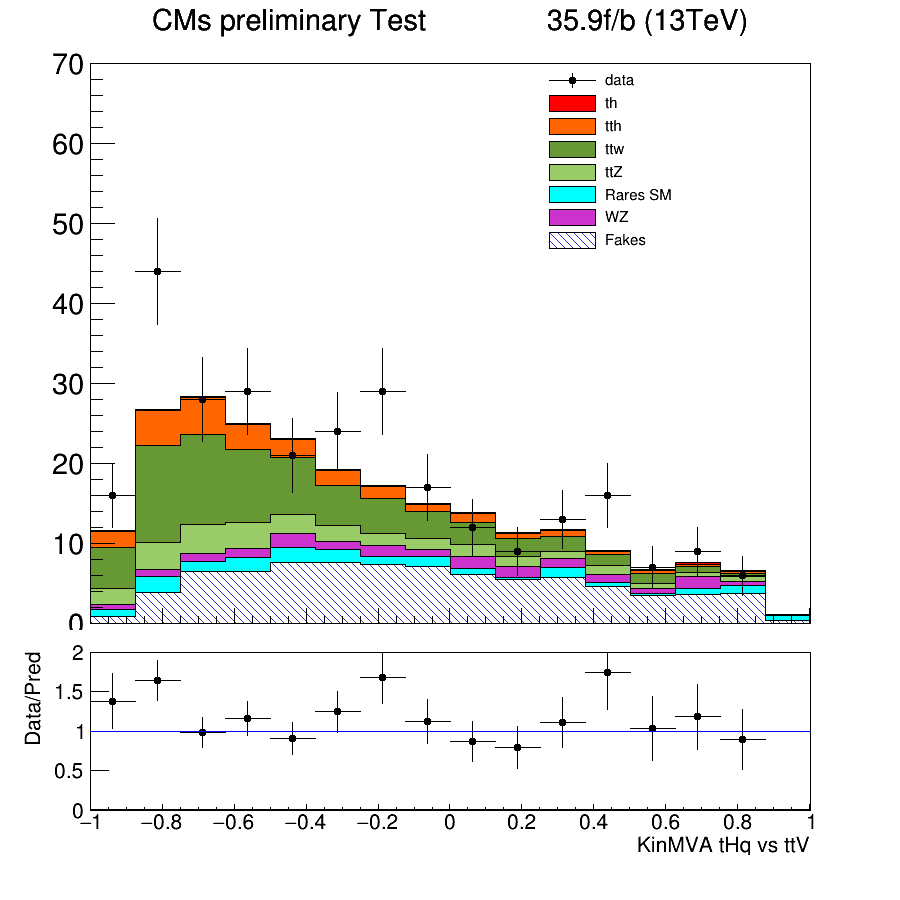
\includegraphics[scale=0.3]{figures/kin.png}
\end{center}
\end{figure}
\end{frame}
\end{document}